
\chapter{Instrument kalibrering}

Alle instrumenter har minst en \textit{inngang} og en \textit{utgang}. For en trykksensor vil inngangen være trykket i et fluid og utgangen er ofte et 4-20mA strømsignal. For en sløyfetester vil inngangen være 4-20mA og utgangen et display som kan leses. 

\textit{Kalibrering} og \textit{valg av måleområde} er to ulike oppgaver som må gjøres for å etablere ønsket og korrekt samsvar mellom et instrument sin inngang og utgang. Kalibrering vil si sørge for at instrumentet måler den fysiske variabelen korrekt. Valg av måleområde sørger for ønsket samsvar mellom inngang og utgang. 





\filbreak
\section{Kalibrering og justering av måleområde}

Justering av måleområde vil si å sette opp hvilke verdier, på inngangen, som  skal vi min- og max utgangssignal. En trykktransmitter kan f.eks. ha et måleområde fra 0 til 20 bar (0 bar = 4mA : 20 bar = 20mA) men vi bestemmer oss for å justere måleområde til å være 0 til 15 bar (0 bar = 4mA :15 bar = 20mA)

Å kalibrere et instrument betyr å sjekke, og eventuelt justere (om nødvendig), responsen slik at utgangen stemmmer nøyaktig med inngangen i det valgte måleområde. For å gjøre dette må en tilføre inngangen på instrumentet en kjent og nøyaktig verdi. For trykktransmitter vil dette si at en må tilføre et kjent og nøyaktig trykk. Dette gjøres ofte med et trykkalibreringsinstrument som har 3-4 ganger bedre nøyaktighet en hva som kreves av målingen. Det er ikke mulig å kalibrere uten å tilføre en kjent fysisk påvirkning til instrumentets inngang. 

På analoge instrumenter vil en justering av måleområde som regel kreve en om kalibrering. Dette er på grunn av  at det er de to skruene Zero og Range(span) som brukes til begge formål. Digitale instrumenter har separate justeringer for hvert av disse formålene. Det er derfor viktig å vite forskjellen. 





\filbreak
\section{Zero og span justeringer på analoge instrumenter}

Hensikten med \textit{kalibrering} er å sørge for at inn- og utgangen på et instrument stemmer overens i hele måleområdet. Hva som menes med dette kan vises i en graf som viser hvordan inngangen  og utgangen skal forholede seg tilhverandre. For de aller fleste instrumenter vil dette forholdet være linært. Det vil si at vi har en rett linje i grafen. 


$$\includegraphics{calibrate01.eps}$$

Denne grafen viser hvordan en prosent av inngangen skal stemmed med samme prosent av utgangen, hele veien fra 0\% til 100\% 

\filbreak

Det blir litt mer komplisert når inn- og utgangs aksene viser enheten som brukes istedenfor prosent. Ta f.eks. en \textit{trykktransmitter}, det er et instrument som skal gjøre om et trykk i gass eller væske til et signal på utgangen av transmitteren, ofte 4-20mA. Her vises en graf for en trykktransmitter med et måleområde på inngangen på 0-100 bar og et elektronisk utgangssignal på 4-20mA. 


$$\includegraphics{calibrate02.eps}$$

Selv om grafen fremdeles er linær, er ikke lengre null trykk tilsvarende null strøm. Dette kalles et aktivt nullpunkt, fordi null trykk på inngangen tilsvarer en strøm på utgangen som ikke er null. 0 bar er LRV på inngangen mens LVR for utgangen er 4mA og ikke 0mA. 

Enhver linær matematisk funkson kan beskrives med formelen:


$$y = mx + b$$

\noindent
Where,

$y$ = Vertikal posisjon på grafen.

$x$ = Horisontal posisjon på grafen. 

$m$ = Stigningen til grafen

$b$ = Punktet der grafen skjærer igjennom y aksen. 

\vskip 10pt


Dette instrumentet sin kalibrering er det samme. Om vi lar $x$ representere instrumentets inngang i bar og $y$ representerer utgangen i milliampere, kan vi skrive følgende formel for dette instrumentet som følger:


$$y = 0.16x + 4$$

På selve instrumetet (trykktransmitteren) er det to justeringer som lar oss tilpasse instrumentet respons til denne ideelle formelen. Den dene justeringen kalles \textit{zero} mens den andre kalles \textit{span} eller av og til \textit{range} alt eller produsent. Disse to justeringene stemmer overens med uttrykkene $b$ og $m$ i formelen for en linær funksjon: zero justeringen flytter instrumentets funksjon  vertikalt langs y-aksen, mens "span" justerer grafens stigning. Ved å justere zero og span kan vi justere instrumentets respons innenfor dets grenser. 


\vskip 10pt

\filbreak

\noindent
Zero adjustments typically take one or more of the following forms in an instrument:

\begin{itemize}
\item Bias force (spring or mass force applied to a mechanism)
\item Mechanical offset (adding or subtracting a certain amount of motion)
\item Bias voltage (adding or subtracting a certain amount of potential)
\end{itemize}

\filbreak

\noindent
Span adjustments typically take one of these forms:

\begin{itemize}
\item Fulcrum position for a lever (changing the force or motion multiplication)
\item Amplifier gain (multiplying or dividing a voltage signal)
\item Spring rate (changing the force per unit distance of stretch)
\end{itemize}

Det er viktig å merke seg at for de fleste instrumenter, vil zero og span justeringer påvirker hverandre. Det vil si at om en justerer en av de vil dette påvirke den andre. Dette gjelder spesielt span da denne nesten alltid påvirker zero. En justering av zero vil ikke alltid påvirke spen. Det er derfor viktig å vite at ved justering av analoge instrumenter må en gå frem og tilbake mellom zero og span til ønsket resultat er oppnådd. 

 



\filbreak
\section{Kalibreringsfeil og testing}

Å effektivt kunne indentifisere og rette opp kalibreringsfeil er viktig for en automatikker. For noen automatikkere spesielt de som jobber i industrier der caliberingsnøyaktivhet er et krav etter loven. Vil kalibrering være noe som tar det meste av tiden dere. For andre automatikere vil kalibrering være noe som utføres en gang i blant. Det er uansett viktig å rette opp kalibreringsfeil raskt og effektivt. Denne seksjonen beskriver noen vanlige kalibreringsfeil og hvor rutiner for å rette dem opp. 




\filbreak
\subsection{Typsike kalibreringsfeil}

Husk at formelen for en rett linje beskriver overføringsfunksjone for alle linære instrumneter. 


$$y = mx + b$$

\noindent
Her er,

$y$ = Output

$m$ = Span justering

$x$ = Input

$b$ = Zero justering

\vskip 10pt

En \textit{zero shift} kalibreringsfeil flytter funksonen vertikalt på grafen, som er det samme som at $b$ verdien i formelen er feil. Dette påvirker alle punkter på grafen likt, noe som gjør at den prosentvise feilen er lik for hele måleområdet. Her et eksempel for en trykktransmitter med et måleområde på inngangen på 0-100 bar og utgangen 4-20mA. 

A \textit{zero shift} calibration error shifts the function vertically on the graph, which is equivalent to altering the value of $b$ in the slope-intercept equation.  This error affects \textit{all} calibration points equally, creating the same percentage of error across the entire range.  Using the same example of a pressure transmitter with 0 to 100 PSI input range and 4 to 20 mA output range: \index{Zero shift}

$$\includegraphics{calibrate06.eps}$$

Om en transmitter har zero shift feil, kan denne feilen rettes opp i ved å justere zero til responsen er innenfor kravene. Dette er det samme som å forandre på $b$ verdien i formelen for en rett linje. 


\filbreak

\textit{Span shift} kalibreringsfeil eller forsterkningsfeil på transmitteren er det sammes om å forandre stigningen $m$ i formelen for en rett linje. Effekten av denne feilen vil ikke være lik i noen del av måleområdet. 


$$\includegraphics{calibrate07.eps}$$

Om en transmitter har feil span eller span kalibreringsfeil, kan en  rette opp i dette ved å justere span til responsen er innenfor kravet. Husk at span som regel påvirker zero slik at du nok blir nødt til å justere begge. Dette er det samme som å justere $m$ i formelen for en rett linje. 


\filbreak

Om en transmitter har linearitetsfeil vil ikke overføringsfunksjon lengre være en rett linje. Denne type feil kan ikke rettes med zero og span justeringer.

$$\includegraphics{calibrate08.eps}$$

Noen instumenter har justeringer for linearitet. Denne justeringen må i tilfellet gjøres i nøye samsvar med manualen til produsenten. Noen instrumenter vil ikke ha en slik justering, det beste du da kan gjøre er å fordele feilen innenfor måleområde slik du kommer innenfor kravet til feilprosent. 


\filbreak

Hysteresefeil er kalibreringsfeil der transmitteren reagerer forskjelling alt etter om den mottar stigende eller synkende verdier. Den eneste måten å oppdage slike feil på er å gjøre en opp/ned test av transmitteren. Det vil si at den bruker det samme målepunktene når en går opp i verdi som når en går ned. 


$$\includegraphics{calibrate09.eps}$$

Hysteresefeil kommer som regel alltid av mekanisk friksjon på en beveglig del eller slark i koblingen mellom mekaniske deler. Friksjon virker alltid i motsatt retning av bevegelsen, hysteresefeil vil derfor alltid ligge etter inngangssignalet. Hysteresefeil kan ikke rettes opp i ved justeringer på instrumentet, det er som regel en mekaniske komponent som må byttes eller smøres. 

\vskip 10pt

I praksis vil de fleste kalibreringsfeil være en kombinasjon av zero, span, linearitet og hysteresefeil. Det er viktig å huske at med få unntak, zero feil kominers som regel med andre feil. Det er ekstremt skjelden en finner en transmitter med span, linearitet eller hysteresefeil som ikke også har en zero feil. Dette gjør at om et instrument stemmer i ett punkt, vil det som regel stemme i alle punkter. Om det ikke gjør det, er det på tide med en rekalibrering. 


\filbreak

Et vanlig testpunkt for automatikere å utføre på en DP-celle er å lukke begge ventiler på manifolden og åpne utlingningsventilen og å tilføre et kjent differansetrykk på 0 bar. 


$$\includegraphics{pressure72.eps}$$

De fleste DP-celler har 0 bar i måleområdet, noe som gjør dette til en enkel enpunkts test. Om denne testen er ok er instrumentet sansynligvis ok over hele måleområdet. Om det ikke er ok må instrumentet rekalibreres. 












\filbreak
\subsection{As-found og as-left dokumentasjon}

Et viktig printsipp ved kalibrering er å dokumentere interumenters som de ble funnet (as-found) og som forlatt (as-left) etter justering. Hensikten med å dokumentere begge er å lage data som gjøre det mulig å kalkulere hvor mye instrumentet driver over tid. Dette er ikke mulig med bare en av disse. Om et instrument driver mye over tid kan dette være en indikator på at instrumentet snart blir defekt. Dette kan være nyttig for prevantivt vedlikehold av instrumentparken. 


Et vanlig format for å dokumentere as-found og as-left data er en tabell som viser kalibreringspunktene, ideell respons og faktisk respons og kalkulert feil for hvert punkt. Her vises et eksempel for en transmitter med et måleområde på 0-200 PSI med 5 testpunkter. 


% No blank lines allowed between lines of an \halign structure!
% I use comments (%) instead, so Tex doesn't choke.

$$\vbox{\offinterlineskip
\halign{\strut
\vrule \quad\hfil # \ \hfil & 
\vrule \quad\hfil # \ \hfil & 
\vrule \quad\hfil # \ \hfil & 
\vrule \quad\hfil # \ \hfil & 
\vrule \quad\hfil # \ \hfil \vrule \cr
\noalign{\hrule}
%
% First row
\textbf{Percent} & \textbf{Input} & \textbf{Output current} & \textbf{Output current} & \textbf{Error} \cr
%
\textbf{of range} & pressure & (ideal) & (measured) & (percent of span) \cr
%
\noalign{\hrule}
%
% Another row
0\% & 0 PSI & 4.00 mA &  & \cr
%
\noalign{\hrule}
%
% Another row
25\% & 50 PSI & 8.00 mA &  & \cr
%
\noalign{\hrule}
%
% Another row
50\% & 100 PSI & 12.00 mA &  & \cr
%
\noalign{\hrule}
%
% Another row
75\% & 150 PSI & 16.00 mA &  & \cr
%
\noalign{\hrule}
%
% Another row
100\% & 200 PSI & 20.00 mA &  & \cr
%
\noalign{\hrule}
} % End of \halign 
}$$ % End of \vbox

Dette bildet viser en enkeltpunkts As-Found kalibrerings  rapport for en temperaturtransmitter. Den viser temperaturen for calibreringsstandarden ($-78.112$ degrees Celsius), temperaturen som instrumentet viste under testen (IUT, $-79$ degrees Celsius) og forskjellen mellom de to ($-0.888$ degrees Celsius)


$$\includegraphics[width=3in]{calibrate28.eps}$$

Legg merket til fortegnet til avviket. Her er det negativt siden responsen er mindre en den skulle vært. Når feilen skal gis i prosent av span blir formelen:


$$\hbox{Error} = {\hbox{IUT} - \hbox{Standard} \over \hbox{Span}} \times 100\%$$




\filbreak
\subsection{Test med stigende og synkende verdier}

Det er ikke uvanlig at en bruker flere kalibreringspunkter, og at en testet med stigende og synkende verdier. 5 punkts kalibrering er en valig standard. I dette eksempelet vises en transmitter med max hysterese på 0.313 \%. Hensikten med opp/ned test er å avdekker hysterese- og dødbåndsfeil. 

% No blank lines allowed between lines of an \halign structure!
% I use comments (%) instead, so Tex doesn't choke.

$$\vbox{\offinterlineskip
\halign{\strut
\vrule \quad\hfil # \ \hfil & 
\vrule \quad\hfil # \ \hfil & 
\vrule \quad\hfil # \ \hfil & 
\vrule \quad\hfil # \ \hfil & 
\vrule \quad\hfil # \ \hfil \vrule \cr
\noalign{\hrule}
%
% First row
\textbf{Percent} & \textbf{Input} & \textbf{Output current} & \textbf{Output current} & \textbf{Error} \cr
%
\textbf{of range} & pressure & (ideal) & (measured) & (percent of span) \cr
%
\noalign{\hrule}
%
% Another row
0\% & 0 PSI & 4.00 mA & 3.99 mA & $-0.0625$ \% \cr
%
\noalign{\hrule}
%
% Another row
25\% $\uparrow$ & 50 PSI & 8.00 mA & \textbf{7.98 mA} & \textbf{$-$0.125 \%} \cr
%
\noalign{\hrule}
%
% Another row
50\% $\uparrow$ & 100 PSI & 12.00 mA & 11.99 mA & $-0.0625$ \% \cr
%
\noalign{\hrule}
%
% Another row
75\% $\uparrow$ & 150 PSI & 16.00 mA & 15.99 mA & $-0.0625$ \% \cr
%
\noalign{\hrule}
%
% Another row
100\% $\uparrow$ & 200 PSI & 20.00 mA & 20.00 mA & 0 \% \cr
%
\noalign{\hrule}
%
% Another row
75\% $\downarrow$ & 150 PSI & 16.00 mA & 16.01 mA & +0.0625 \% \cr
%
\noalign{\hrule}
%
% Another row
50\% $\downarrow$ & 100 PSI & 12.00 mA & 12.02 mA & +0.125 \% \cr
%
\noalign{\hrule}
%
% Another row
25\% $\downarrow$ & 50 PSI & 8.00 mA & \textbf{8.03 mA} & \textbf{+0.188 \%} \cr
%
\noalign{\hrule}
%
% Another row
0\% $\downarrow$ & 0 PSI & 4.00 mA & 4.01 mA & +0.0625 \% \cr
%
\noalign{\hrule}
} % End of \halign 
}$$ % End of \vbox

Legg igjen merke til at feilen er enten negativ eller positiv alt etter om den målte verdien er over eller under ønsket verdi. Veridene i denne tabellen som er oppgitt i prosent av span er utregnet med denne formelen:
$$\hbox{Error} = \left( {{I_{measured} - I_{ideal}} \over 16 \hbox{ mA}} \right)  \left( 100 \% \right)$$

Ved utførelsen av opp/ned test er det viktig å ikke gå over noen av testpunktene. Om du havner over et av punktene må du gå litt tilbake og nærme deg testpuniktet på samme måte som før. Om du ikke klarer dette vil du ikke kunne si noe om hysterese- og dødbåndsfeil







\filbreak
\subsection{Automated calibration}

Maintaining the calibration of instruments at a large industrial facility is a daunting task.  Aside from the actual labor of checking and adjusting calibration, records must be kept not only of instrument performance but also of test conditions and criteria (e.g. calibration tolerance, time interval between calibrations, number of points to check, specific procedures, etc.).  Any practical method to minimize human error in this process is welcome.  For this reason, automated and semi-automated calibration tools have been developed to help manage the data associated with calibration, and to make the instrument technician's job more manageable.  

An example of a fully automated calibration system is a process chemical analyzer where a set of solenoid valves direct chemical samples of known composition to the analyzer at programmed time intervals, a computer inside the analyzer recording the analyzer's error (compared to the known standard) and auto-adjusting the analyzer in order to correct for whatever errors are detected.  In the following illustration we see a schematic of a gas analyzer with two compressed-gas cylinders holding gases of 0\% and 100\% concentration of the compound(s) of interest, called ``zero gas'' and ``span gas'', connected through solenoid valves so that the chemical analyzer may be automatically tested against these standards:  \index{Calibration gas}  \index{Gas, calibration}

$$\includegraphics{calibrate15.eps}$$

The only time a human technician need attend to the analyzer is when parameters not monitored by the auto-calibration system must be checked, and when the auto-calibration system detects an error too large to self-correct (thus indicating a fault).

\filbreak

An example of a semi-automated calibration system is an instrument such as Fluke's series of \textit{Documenting Process Calibrators} (DPC).  These devices function as standards for electrical measurements such as voltage, current, and resistance, with built-in database capability for storing calibration records and test conditions:  \index{Documenting calibrator}  \index{Fluke model 744 Documenting Process Calibrator (DPC)}

$$\includegraphics[height=4in]{calibrate29.eps}$$

A technician using a documenting calibrator such as this is able to log As-Found and As-Left data in the device's memory and download the calibration results to a computer database at some later time.  The calibrator may also be programmed with test conditions for each specific instrument on the technician's work schedule, eliminating the need for that technician to look up each instrument's test conditions in a book, and thereby reducing the potential for human error.  

\filbreak

An example of database software used to schedule routine instrument calibrations and archive the results is Fluke's \textit{DPCTrack2}, a point-and-click user interface serving as a front-end to an SQL database where the instrument data is maintained in digital format on the computer's hard drive:  \index{Fluke DPCTrack2 calibration management software}

$$\includegraphics{calibrate30.eps}$$

Calibration management software allows managers to define calibration schedules, tolerances, and even technician work assignments, the software allowing for downloading of this setup information into a hand-held calibrator unit, as well as uploading and archival of calibration results following the procedure.  \index{Calibration management software}

\vskip 10pt

In some industries, this degree of rigor in calibration record-keeping is merely helpful; in other industries it is vital for business.  Examples of the latter include pharmaceutical manufacturing, where regulatory agencies (such as the Food and Drug Administration in the United States) enforces rigorous standards for manufacturing quality including requirements for frequent testing and data archival of process instrument accuracy.  Record-keeping in such industries is not limited to As-Found and As-Left calibration results, either; each and every action taken on that instrument by a human being must be recorded and archived so that a complete audit of causes may be conducted should there ever be an incident of product mis-manufacture.  \index{Fluke Documenting Process Calibrator (DPC) instruments}








\filbreak
\section{Damping adjustments}

\label{transmitter_damping}

The vast majority of modern process transmitters (both analog and digital) come equipped with a feature known as \textit{damping}.  This feature is essentially a low-pass filter function placed in-line with the signal, reducing the amount of process ``noise'' reported by the transmitter.  \index{Damping}

Imagine a pressure transmitter sensing water pressure at the outlet of a large pump.  The flow of water exiting a pump tends to be extremely turbulent, and any pressure-sensing device connected to the immediate discharge port of a pump will interpret this turbulence as fluctuations in pressure.  This means the pressure signal output by the transmitter will fluctuate as well, causing any indicator or control system connected to that transmitter to register a ``noisy'' water pressure:

$$\includegraphics{calibrate16.eps}$$

Such ``noise'' wreaks havoc with most forms of feedback control, since the control system will interpret these rapid fluctuations as real pressure changes requiring corrective action.  Although it is possible to configure some control systems to ignore such noise, the best solution is to correct the problem at the source either by relocating the pressure transmitter's impulse line tap to a place where it will not be exposed to so much turbulence, or somehow prevent that sensed turbulence from being represented in the transmitter's signal.

Since this noise is of a much greater frequency than the normal cycles of pressure in a process system, it is relatively easy to reduce the amount of noise in the transmitter signal simply by filtering that electronic signal using a low-pass filter circuit.  

\filbreak

The simplest low-pass filter circuit is nothing more than a resistor and capacitor:

$$\includegraphics{calibrate17.eps}$$

Low-frequency voltage signals applied to this circuit emerge at the output terminal relatively unattenuated, because the reactance of the capacitor is quite large at low frequencies.  High-frequency signals applied to the same circuit become attenuated by the capacitor, which tends to ``short'' those signals to ground with its low reactance to high frequencies.  The performance of such a filter circuit is primarily characterized by its \textit{cutoff frequency}, mathematically defined as $f = {1 \over 2 \pi RC}$.  The cutoff frequency is the point at which only 70.7\% of the input signal appears at the output (i.e. a $-3$ dB attenuation in voltage).

If successfully applied to a process transmitter, such low-pass filtering has the effect of ``quieting'' an otherwise noisy signal so only the real process pressure changes are seen, while the effect of turbulence (or whatever else was causing the noise) becomes minimal.  In the world of process control, the intentional low-pass filtering of process measurement signals is often referred to as \textit{damping} because its effect is to ``damp'' (attenuate) the effects of process noise:

$$\includegraphics{calibrate18.eps}$$

\filbreak

In order for damping to be a useful tool for the technician in mitigating measurement noise, it must be adjustable.  In the case of the RC filter circuit, the degree of damping (cutoff frequency) may be adjusted by changing the value or either $R$ or $C$, with $R$ being the easier component to adjust.  This next photograph shows the location of an adjustable resistance on the printed circuit board of a Rosemount model 1151 analog pressure transmitter:

$$\includegraphics[width=3in]{calibrate34.eps}$$

In digital transmitters where the damping is performed by a digital algorithm\footnote{Various digital damping algorithms exist, but it may take as simple a form as successive averaging of buffered signal values coming out of a first-in-first-out (``FIFO'') shift register.}, damping may be adjusted by setting a numerical value in the transmitter's configuration parameters.  In pneumatic transmitters, damping could be implemented by installing viscous elements to the mechanism, or more simply by adding volume to the signal line (e.g. excess tubing length, larger tubing diameter, or even ``capacity tanks'' connected to the tube for increased volume).  \index{Capacity tank}  \index{Digital damping}  \index{Damping, digital algorithm}  \index{FIFO shift register}  \index{Shift register, FIFO}

The key question for the technician then becomes, ``how much damping should be applied?''  Insufficient damping will allow too much noise to reach the control system (causing ``noisy'' trends, indications, and erratic control), while excessive damping will cause the transmitter to understate the significance of sudden (real) process changes.  In my experience there is a bad tendency for instrument technicians to apply excessive damping in transmitters.  A transmitter with too much damping (i.e. cutoff frequency set too low, or time constant value set too high) causes the trend graph to be very smooth, which at first appears to be a good thing.  After all, the whole point of a control system is to hold the process variable tightly to setpoint, so the appearance of a ``flat line'' process variable trend is enticing indeed.  However, the problem with excessive damping is that the transmitter gives a sluggish response to any sudden changes in the real process variable.  

\filbreak

A dual-trend graph of a pressure transmitter experiencing a sudden increase in process pressure shows this principle, where the undamped transmitter signal is shown in the upper portion and the over-damped signal in the lower portion (please note the vertical offset between these two trends is shown only for your convenience in comparing the two trend shapes):

$$\includegraphics{calibrate19.eps}$$

Excessive damping causes the transmitter to ``lie'' to the control system by reporting a process variable that changes much slower than it actually does.  The degree to which this ``lie'' adversely affects the control system (and/or the human operator's judgment in manually responding to the change in pressure) depends greatly on the nature of the control system and its importance to the overall plant operation.  

One way damping may cause control problems is in systems where the loop controller is aggressively tuned.  In such systems, even relatively small amounts of damping may cause the actual process variable to overshoot setpoint because the controller ``thinks'' the process variable is responding too slowly and takes action to speed its response.  A common example of this is liquid flow control, where the process variable signal is typically ``noisy'' and the control action is typically aggressive.  A technician may introduce damping to the transmitter with good intent, but unexpectedly causes the control system to wildly overshoot setpoint (or even oscillate) because the controller is trying to get a ``sluggish'' process variable to respond quicker than the transmitter filtering will allow the signal to change.  In reality, the process variable (fluid flow rate) is not sluggish at all, but only appears that way because the transmitter is damped.  What is worse, this instability will \textit{not} appear on a trend of the process variable because the control system never sees the real process variable, but only the ``lie'' reported by the over-damped transmitter.  If any rule may be given as to how much damping to use in any transmitter, it is this: use as \textit{little} as necessary to achieve good control.

Damping should be set to absolute minimum during calibration, so the results of applying stimuli to the transmitter will be immediately seen by the technician.





\filbreak
\section{LRV og URV innstillinger, digital trim (digitale transmittere)}

Innføringen av "smarte" feltinstrumenter som inneholder mikroprosessorer har vært et stort fremskrit for instrumenteringsbransjen. Disse instrumentene har innebygget diagnostikk, større nøyaktighet(på grunn av mulighet for å kompensere for sensor ulineariteteter), og muligheten for å kommunisere digitalt med styresystemer for å rapportere ulike parametre. 


Et forenklet blokkdiagram over en "smart" transmitter kan se slik ut:

$$\includegraphics{calibrate03.eps}$$

\filbreak

Legg merke til alle justeringene på denne trype transmitter i forhold til en forholdsvis enkel analog tranmitter:

$$\includegraphics{calibrate04.eps}$$

Note how the only calibration adjustments available in the analog transmitter are the ``zero'' and ``span'' settings.  This is clearly not the case with smart transmitters.  Not only can we set lower- and upper-range values (LRV and URV) in a smart transmitter, but it is also possible to calibrate the analog-to-digital and digital-to-analog converter circuits independently of each other.  What this means for the calibration technician is that a full calibration procedure on a smart transmitter potentially requires more work and a greater number of adjustments than an all-analog transmitter\footnote{Although those adjustments made on a digital transmitter tend to be easier to perform than repeated zero-and-span adjustments on analog transmitters due to the inevitable ``interaction'' between analog zero and span adjustments requiring repeated checking and re-adjustment during the calibration period.}. \index{LRV} \index{URV} \index{Lower range value} \index{Upper range value} 

A common mistake made among students and experienced technicians alike is to confuse the range settings (LRV and URV) for actual calibration adjustments.  Just because you digitally set the LRV of a pressure transmitter to 0.00 PSI and the URV to 100.00 PSI does not necessarily mean it will register accurately at points within that range!  The following example will illustrate this fallacy.

Suppose we have a smart pressure transmitter ranged for 0 to 100 PSI with an analog output range of 4 to 20 mA, but this transmitter's pressure sensor is fatigued from years of use such that an actual applied pressure of 100 PSI generates a signal that the analog-to-digital converter interprets as only 96 PSI\footnote{A 4\% calibration error caused by sensor aging is enormous for any modern digital transmitter, and should be understood as an exaggeration presented only for the sake of illustrating how sensor error affects overall calibration in a smart transmitter.  A more realistic amount of sensor error due to aging would be expressed in small fractions of a percent.}.  Assuming everything else in the transmitter is in perfect condition, with perfect calibration, the output signal will still be in error:

$$\includegraphics{calibrate05.eps}$$

As the saying goes, ``a chain is only as strong as its weakest link.''  Here we see how the calibration of the most sophisticated pressure transmitter may be corrupted despite perfect calibration of both analog/digital converter circuits, and perfect range settings in the microprocessor.  The microprocessor ``thinks'' the applied pressure is only 96 PSI, and it responds accordingly with a 19.36 mA output signal.  \textit{The only way anyone would ever know this transmitter was inaccurate at 100 PSI is to actually apply a known value of 100 PSI fluid pressure to the sensor and note the incorrect response.}  The lesson here should be clear: digitally setting a smart instrument's LRV and URV points does \textit{not} constitute a legitimate calibration of the instrument.

For this reason, smart instruments always provide a means to calibrate both the ADC and DAC circuits, to ensure the microprocessor ``sees'' the correct representation of the applied stimulus and to ensure the microprocessor's output signal gets accurately converted into a DC current, respectively.  This calibration function is called \textit{digital trim}.

\filbreak

A convenient way to test a digital transmitter's analog/digital converters is to monitor the microprocessor's process variable (PV) and analog output (AO) registers while comparing the real input and output values against trusted calibration standards.  A HART communicator device\footnote{HART is a hybrid analog/digital communication protocol used by a great many field instruments, allowing maintenance personnel to access and edit digital parameters inside the instrument using a computer-based interface.  Hand-held HART communicators exist for this purpose, as does HART software designed to run on a personal computer.  HART modems also exist to connect personal computers to HART-compatible field instruments.} provides this ``internal view'' of the registers so we may see what the microprocessor ``sees.''  The following example shows a differential pressure transmitter with a sensor (analog-to-digital) calibration error:

$$\includegraphics{calibrate26.eps}$$

Here, the calibration standard for pressure input to the transmitter is a digital pressure gauge, registering 25.00 inches of water column.  The digital multimeter (DMM) is our calibration standard for the current output, and it registers 11.93 milliamps.  Since we would expect an output of 12.00 milliamps at this pressure (given the transmitter's range values of 0 to 50 inches W.C.), we immediately know from the pressure gauge and multimeter readings that some sort of calibration error exists in this transmitter.  Comparing the HART communicator's displays of PV and AO against our calibration standards reveals more information about the nature of this error: we see that the AO value (11.930 mA) agrees with the multimeter while the PV value (24.781 "W.C.) does \textit{not} agree with the digital pressure gauge.  This tells us the calibration error lies within the sensor (input) of the transmitter and not with the DAC (output).  Thus, the correct calibration procedure to perform on this errant transmitter is a \textit{sensor trim}.

\filbreak

In this next example, we see what an output (DAC) error would look like with another differential pressure transmitter subjected to the same test:

$$\includegraphics{calibrate27.eps}$$

Once again, the calibration standard for pressure input to the transmitter is a digital pressure gauge, registering 25.00 inches of water column.  A digital multimeter (DMM) still serves as our calibration standard for the current output, and it registers 11.93 milliamps.  Since we expect 12.00 milliamps output at this pressure (given the transmitter's range values of 0 to 50 inches W.C.), we immediately know from the pressure gauge and multimeter readings that some sort of calibration error exists in this transmitter (just as before).  Comparing the HART communicator's displays of PV and AO against our calibration standards reveals more information about the nature of this error: we see that the PV value (25.002 inches W.C.) agrees with the digital pressure gauge while the AO value (12.001 mA) does \textit{not} agree with the digital multimeter.  This tells us the calibration error lies within the digital-to-analog converter (DAC) of the transmitter and not with the sensor (input).  Thus, the correct calibration procedure to perform on this errant transmitter is an \textit{output trim}.

Note how in both scenarios it was absolutely necessary to interrogate the transmitter's microprocessor registers with a HART communicator to determine where the error was located.  Merely comparing the pressure and current standards' indications was not enough to tell us any more than the fact we had some sort of calibration error inside the transmitter.  Not until we viewed the microprocessor's own values of PV and AO could we determine whether the calibration error was related to the ADC (input), the DAC (output), or perhaps even both.

\vskip 10pt

\filbreak

Sadly, I have witnessed technicians attempt to use the LRV and URV settings in a manner not unlike the zero and span adjustments on an analog transmitter to correct errors such as these.  While it may be possible to get an out-of-calibration transmitter to yield correct output current signal values over its calibrated range of input values by skewing the LRV and URV settings, it defeats the purpose of having separate ``trim'' and ``range'' settings inside the transmitter.  Also, it causes confusion if ever the control system connected to the transmitter interrogates process variable values digitally rather than interpreting it via the 4-20 mA loop current signal.  Finally, ``calibrating'' a transmitter by programming it with skewed LRV/URV settings corrupts the accuracy of any intentionally nonlinear functions such as square-root characterization (used for flow measurement applications) or strapping tables (used for liquid level measurement applications in vessels where the cross-sectional area varies with liquid height).

Once digital trims have been performed on both input and output converters, of course, the technician is free to re-range the microprocessor as many times as desired without re-calibration.  This capability is particularly useful when re-ranging is desired for special conditions, such as process start-up and shut-down when certain process variables drift into uncommon regions.  An instrument technician may use a hand-held HART communicator device to re-set the LRV and URV range values to whatever new values are desired by operations staff without having to re-check calibration by applying known physical stimuli to the instrument.  So long as the ADC and DAC trims are both correct, the overall accuracy of the instrument will still be good with the new range.  With analog instruments, the only way to switch to a different measurement range was to change the zero and span adjustments, which \textit{necessitated} the re-application of physical stimuli to the device (a full re-calibration).  Here and here alone we see where calibration is not necessary for a smart instrument.  If overall measurement accuracy must be verified, however, there is no substitute for an actual physical calibration, and this entails both ADC and DAC ``trim'' procedures for a smart instrument.

\vskip 10pt

Completely digital (``Fieldbus'') transmitters are similar to ``smart'' analog-output transmitters with respect to distinct trim and range adjustments.  For an explanation of calibration and ranging on FOUNDATION Fieldbus transmitters, refer to section \ref{FF transmitter calibration} beginning on page \pageref{FF transmitter calibration}.









\filbreak
\section{An analogy for calibration versus ranging}

\label{calibration_versus_ranging}

The concepts of \textit{calibration} (trimming) and \textit{ranging} are often difficult for new students of instrumentation to immediately grasp.  A simple analogy useful for understanding these topics is that of setting a digital alarm clock.

Suppose you purchase a digital alarm clock to wake you up at 7:00 AM in the morning so that you can get to school on time.  It would be foolish to simply unpack your new clock from its box, power it up, and set the wake-up time to 7:00 AM expecting it will wake you at the correct time.  Before \textit{trusting} this alarm time of 7:00 AM, you would first have to synchronize your new clock to some standard time source (such as the time broadcast by your local telephone service, or better yet the shortwave radio broadcast of WWV or WWVH\footnote{The NIST broadcasts audio transmissions of ``Coordinated Universal Time'' (UTC) on the shortwave radio frequencies 5 MHz, 10 MHz, 15 MHz, 20 MHz, and 25 MHz.  Announcements of time, in English, occur at the top of every minute.}) so that it accurately registers time for the zone in which you live.  Otherwise, the wake-up setting of 7:00 AM will be hopelessly uncertain.

Once your clock is synchronized against a trusted time source, however, the wake-up (alarm) time may be set at will.  If your class schedule changed, allowing one more hour of sleep, you could re-set the wake-up time from 7:00 AM to 8:00 AM without any need to re-synchronize (re-calibrate) the clock.  The only reason for re-synchronizing your clock to the time standard is to compensate for inevitable \textit{drift} due to imperfections in the clock circuitry.

Synchronizing the clock to a standard time source is analogous to ``calibrating'' or ``trimming'' a smart transmitter: you are establishing an accurate correspondence between what the device's microprocessor \textit{perceives} and what the actual (real-life) values \textit{are}.  This step need only be done at the very beginning of the device's service, and every so often as warranted by the device's calibration drift over time\footnote{In the case of pressure transmitters, re-trimming may be necessary if the device is ever re-mounted in a different orientation.  Changing the physical orientation of a pressure transmitter alters the direction in which gravity tugs on the sensing element, causing it to respond as though a constant bias pressure were applied to it.  This bias is often on the order of an inch of water column (or less), and usually consequential only for low-pressure applications such as furnace draft pressure.}.

Setting the wake-up (alarm) time on the clock is analogous to setting the LRV and URV parameters of a smart transmitter: you are defining the \textit{action(s)} taken by the device at certain measured values.  For the alarm clock, you are defining the hour and minute of day when the alarm sounds.  For the transmitter, you are defining the measured variable values at which it will output 4 mA and 20 mA (for a 4-20 mA analog output range).

\vskip 10pt

By contrast, an analog transmitter blends the functions of calibration and ranging into one.  A useful analogy for this is to imagine using a simple wind-up mechanical timer to wake you at 7:00 AM.  Such a crude timing device does not even register time in hours and minutes like a digital alarm clock: instead, it simply counts down time from its starting point and sounds an alarm when the descending count reaches zero.  In order to set this device for a 7:00 AM wake-up alarm, you must first determine the current time and then calculate how many hours the timer must run before the time reaches 7:00 AM (e.g. if you are setting the wind-up alarm when you go to bed at 10:30 PM, this would equate to a timing period of 8.5 hours).

Every single time you set this wind-up alarm, you must consult a time standard to know how many hours and minutes of count-down time to set it for.  If you decide to wake up at a different time in the morning, you must (once again) consult a standard time source, perform the necessary arithmetic, and set the timer accordingly.  Setting the alarm time on this mechanism necessitates re-calibrating it to the local standard time without exception.  Here, there is no distinction between synchronization and alarm setting; no distinction between calibration and ranging -- to do one is to do the other.









\filbreak
\section{Calibration procedures}

As described earlier in this chapter, \textit{calibration} refers to the adjustment of an instrument so its output accurately corresponds to its input throughout a specified range.  The only way we can know that an instrument's output accurately corresponds to its input over a continuous range is to subject that instrument to known input values while measuring the corresponding output signal values.  This means we must use trusted \textit{standards} to establish known input conditions and to measure output\footnote{A noteworthy exception is the case of digital instruments, which output digital rather than analog signals.  In this case, there is no need to compare the digital output signal against a standard, as digital numbers are not liable to calibration drift.  However, the calibration of a digital instrument still requires comparison against a trusted standard in order to validate an analog quantity.  For example, a digital pressure transmitter must still have its input calibration values validated by a pressure standard, even if the transmitter's digital output signal cannot drift or be misinterpreted.} signals.  The following examples show both input and output standards used in the calibration of pressure and temperature transmitters:

$$\includegraphics{calibrate31.eps}$$

\filbreak

$$\includegraphics{calibrate32.eps}$$

%ADD: include examples of other instrument calibrations, with standards:
%ADD:    --> Wireless digital transmitter
%ADD:    --> Pneumatic pressure transmitter
%ADD:    --> Analytical transmitter (e.g. pH, O2)

It is the purpose of this section to describe procedures for efficiently calibrating different types of instruments.

\filbreak
\subsection{Linear instruments}

The simplest calibration procedure for an analog, linear instrument is the so-called \textit{zero-and-span} method.  The method is as follows:

\begin{enumerate}
\item Apply the lower-range value stimulus to the instrument, wait for it to stabilize
\item Move the ``zero'' adjustment until the instrument registers accurately at this point
\item Apply the upper-range value stimulus to the instrument, wait for it to stabilize
\item Move the ``span'' adjustment until the instrument registers accurately at this point
\item Repeat steps 1 through 4 as necessary to achieve good accuracy at both ends of the range
\end{enumerate}

An improvement over this crude procedure is to check the instrument's response at several points between the lower- and upper-range values.  A common example of this is the so-called \textit{five-point calibration} where the instrument is checked at 0\% (LRV), 25\%, 50\%, 75\%, and 100\% (URV) of range.  A variation on this theme is to check at the five points of 10\%, 25\%, 50\%, 75\%, and 90\%, while still making zero and span adjustments at 0\% and 100\%.  Regardless of the specific percentage points chosen for checking, the goal is to ensure that we achieve (at least) the minimum necessary accuracy at all points along the scale, so the instrument's response may be trusted when placed into service. \index{Five-point calibration} \index{5-point calibration}

Yet another improvement over the basic five-point test is to check the instrument's response at five calibration points \textit{decreasing} as well as \textit{increasing}.  Such tests are often referred to as \textit{Up-down} calibrations.  The purpose of such a test is to determine if the instrument has any significant \textit{hysteresis}: a lack of responsiveness to a change in direction.  \index{Up-down calibration test} \index{Hysteresis}

Some analog instruments provide a means to adjust linearity.  This adjustment should be moved only if absolutely necessary!  Quite often, these linearity adjustments are very sensitive, and prone to over-adjustment by zealous fingers.  The linearity adjustment of an instrument should be changed only if the required accuracy cannot be achieved across the full range of the instrument.  Otherwise, it is advisable to adjust the zero and span controls to ``split'' the error between the highest and lowest points on the scale, and leave linearity alone.

\vskip 10pt

\filbreak

The procedure for calibrating a ``smart'' digital transmitter -- also known as \textit{trimming} -- is a bit different.  Unlike the zero and span adjustments of an analog instrument, the ``low'' and ``high'' trim functions of a digital instrument are typically non-interactive.  This means you should only have to apply the low- and high-level stimuli \textit{once} during a calibration procedure.  Trimming the sensor of a ``smart'' instrument consists of these four general steps:

\begin{enumerate}
\item Apply the lower-range value stimulus to the instrument, wait for it to stabilize
\item Execute the ``low'' sensor trim function
\item Apply the upper-range value stimulus to the instrument, wait for it to stabilize
\item Execute the ``high'' sensor trim function
\end{enumerate}

Likewise, trimming the output (Digital-to-Analog Converter, or DAC) of a ``smart'' instrument consists of these six general steps:

\begin{enumerate}
\item Execute the ``low'' output trim test function
\item Measure the output signal with a precision milliammeter, noting the value after it stabilizes
\item Enter this measured current value when prompted by the instrument
\item Execute the ``high'' output trim test function
\item Measure the output signal with a precision milliammeter, noting the value after it stabilizes
\item Enter this measured current value when prompted by the instrument
\end{enumerate}

\vskip 10pt

After both the input and output (ADC and DAC) of a smart transmitter have been trimmed (i.e. calibrated against standard references known to be accurate), the lower- and upper-range values may be set.  In fact, once the trim procedures are complete, the transmitter may be ranged and ranged again as many times as desired.  The only reason for re-trimming a smart transmitter is to ensure accuracy over long periods of time where the sensor and/or the converter circuitry may have drifted out of acceptable limits.  This stands in stark contrast to analog transmitter technology, where re-ranging \textit{necessitates} re-calibration every time.



\filbreak
\subsection{Nonlinear instruments}

The calibration of inherently nonlinear instruments is much more challenging than for linear instruments.  No longer are two adjustments (zero and span) sufficient, because more than two points are necessary to define a curve.

Examples of nonlinear instruments include expanded-scale electrical meters, square root characterizers, and position-characterized control valves.

Every nonlinear instrument will have its own recommended calibration procedure, so I will defer you to the manufacturer's literature for your specific instrument.  I will, however, offer one piece of advice: when calibrating a nonlinear instrument, document all the adjustments you make (e.g. how many turns on each calibration screw) just in case you find the need to ``re-set'' the instrument back to its original condition.  More than once I have struggled to calibrate a nonlinear instrument only to find myself further away from good calibration than where I originally started.  In times like these, it is good to know you can always reverse your steps and start over!





\filbreak
\subsection{Discrete instruments}

The word ``discrete'' means \textit{individual} or \textit{distinct}.  In engineering, a ``discrete'' variable or measurement refers to a true-or-false condition.  Thus, a discrete sensor is one that is only able to indicate whether the measured variable is above or below a specified setpoint. \index{Discrete}

Examples of discrete instruments are \textit{process switches} designed to turn on and off at certain values.  A pressure switch, for example, used to turn an air compressor on if the air pressure ever falls below 85 PSI, is an example of a discrete instrument.

Discrete instruments require periodic calibration just like continuous instruments.  Most discrete instruments have just one calibration adjustment: the \textit{set-point} or \textit{trip-point}.  Some process switches have two adjustments: the set-point as well as a \textit{deadband} adjustment.  The purpose of a deadband adjustment is to provide an adjustable buffer range that must be traversed before the switch changes state.  To use our 85 PSI low air pressure switch as an example, the set-point would be 85 PSI, but if the deadband were 5 PSI it would mean the switch would not change state until the pressure rose above 90 PSI (85 PSI + 5 PSI).

When calibrating a discrete instrument, you must be sure to check the accuracy of the set-point \textit{in the proper direction of stimulus change}.  For our air pressure switch example, this would mean checking to see that the switch changes states at 85 PSI \textit{falling}, not 85 PSI \textit{rising}.  If it were not for the existence of deadband, it would not matter which way the applied pressure changed during the calibration test.  However, deadband will always be present in a discrete instrument, whether that deadband is adjustable or not.

For example, a pressure switch with a deadband of 5 PSI set to trip at 85 PSI falling would re-set at 90 PSI rising.  Conversely, a pressure switch (with the same deadband of 5 PSI) set to trip at 85 PSI rising would re-set at 80 PSI falling.  In both cases, the switch ``trips'' at 85 PSI, but the direction of pressure change specified for that trip point defines which side of 85 PSI the re-set pressure will be found.

A procedure to efficiently calibrate a discrete instrument without too many trial-and-error attempts is to set the stimulus at the desired value (e.g. 85 PSI for our hypothetical low-pressure switch) and then move the set-point adjustment in the \textit{opposite} direction as the intended direction of the stimulus (in this case, \textit{increasing} the set-point value until the switch changes states).  The basis for this technique is the realization that most comparison mechanisms cannot tell the difference between a rising process variable and a falling setpoint (or vice-versa).  Thus, a falling pressure may be simulated by a rising set-point adjustment.  You should still perform an actual changing-stimulus test to ensure the instrument responds properly under realistic circumstances, but this ``trick'' will help you achieve good calibration in less time.





\filbreak
\section{Instrument turndown}

An important performance parameter for transmitter instruments is something often referred to as \textit{turndown} or \textit{rangedown}.  ``Turndown'' is defined as the ratio of maximum allowable span to the minimum allowable span for a particular instrument. \index{Turndown} \index{Rangedown}

Suppose a pressure transmitter has a maximum calibration range of 0 to 300 pounds per square inch (PSI), and a turndown of 20:1.  This means that a technician may adjust the span anywhere between 300 PSI (e.g. range = 0 to 300 PSI) and 15 PSI (e.g. range = 0 to 15 PSI).  This is important to know in order to select the proper transmitter for any given measurement application.  The odds of you finding a transmitter with just the perfect factory-calibrated range for your measurement application may be quite small, meaning you will have to adjust its range to fit your needs.  The turndown ratio tells you how far you will be able to practically adjust your instrument's range.

\vskip 10pt

For example, suppose you were working at a facility where the operations personnel requested a pressure transmitter installed on a process vessel with a measurement range of 50 PSI to 90 PSI.  You go to the warehouse where all the new instruments are stocked, and find a pressure transmitter with a (maximum) range of zero to 1000 PSI, and a turndown ratio of 20:1.  Dividing the maximum span of 1000 PSI by 20, we arrive at a minimum span of 50 PSI.  The span requested by operations for this pressure transmitter is 40 PSI (90 PSI $-$ 50 PSI), which means the transmitter you found in the warehouse will \textit{not} be able to ``turn down'' that far.  At best, we could range it for 50 PSI to 100 PSI, or perhaps for 40 PSI to 90 PSI, but not the 50 PSI to 90 PSI requested by operations.  At this point, you could return to the operations personnel to ask if a 50 PSI span would be acceptable -- if not, you will have to order a different pressure transmitter with a smaller span (or with a greater turndown ratio\footnote{Modern ``smart'' electronic pressure transmitters typically boast turndown ratios exceeding 100:1, with some having turndown ratios of 200:1 or more!  Large turndown ratios are good because they allow users of instrumentation to maintain a smaller quantity of new transmitters in stock, since transmitters with large turndown ratios are more versatile (i.e. applicable to a wider variety of spans) than transmitters with small turndown ratios.}).

\vskip 10pt

Another important consideration with turndown is the \textit{accuracy} of the instrument at the stated turndown.  The further an instrument is ``turned down'' from its maximum span, generally the worse its accuracy becomes at that reduced span.  For example, the Micro Motion ``ELITE'' series of Coriolis mass flowmeters\footnote{According to Emerson product datasheet PS-00374, revision L, June 2009.} are advertised to perform within an accuracy envelope of $\pm$0.05\% at turndown ratios up to 20:1, but that measurement uncertainty increases to $\pm$0.25\% at a turndown of 100:1, and to $\pm$1.25\% at a turndown of 500:1.  It should be noted that the degradation of measurement accuracy at large turndown ratios is not some defect of Micro Motion flowmeters (far from it!), but rather an inescapable consequence of pushing an instrument's turndown to its limit.  \index{Micro Motion ELITE model Coriolis mass flowmeter}





\filbreak
\section{NIST traceability}

As defined previously, \textit{calibration} means the comparison and adjustment (if necessary) of an instrument's response to a stimulus of precisely known quantity, to ensure operational accuracy.  In order to perform a calibration, one must be reasonably sure that the physical quantity used to stimulate the instrument is accurate in itself.  For example, if I try calibrating a pressure gauge to read accurately at an applied pressure of 200 PSI, I must be reasonably sure that the pressure I am using to stimulate the gauge is actually 200 PSI.  If it is not 200 PSI, then all I am doing is adjusting the pressure gauge to register 200 PSI when in fact it is sensing something different.

Ultimately, this is a philosophical question of \underbar{epistemology}: \textit{how do we know what is true?}  There are no easy answers here, but teams of scientists and engineers known as \textit{metrologists} devote their professional lives to the study of calibration standards to ensure we have access to the best approximation of ``truth'' for our calibration purposes.  \textit{Metrology} is the science of measurement, and the central repository of expertise on this science within the United States of America is the \textit{National Institute of Standards and Technology}, or the \textit{NIST} (formerly known as the \textit{National Bureau of Standards}, or \textit{NBS}).  \index{Metrology} \index{NIST}  \index{NBS}  \index{National Bureau of Standards}  \index{National Institute of Standards and Technology}  \index{Epistemology}

Experts at the NIST work to ensure we have means of tracing measurement accuracy back to \textit{intrinsic standards}, which are quantities inherently fixed (as far as anyone knows).  The vibrational frequency of an isolated cesium atom when stimulated by radio energy, for example, is an intrinsic standard used for the measurement of time (forming the basis of the so-called \textit{atomic clock}).  So far as anyone knows, this frequency is fixed in nature and cannot vary: each and every isolated cesium atom has the exact same resonant frequency.  The distance traveled in a vacuum by 1650763.73 wavelengths of light emitted by an excited krypton-86 ($^{86}$Kr) atom is the intrinsic standard for one meter of length.  Again, so far as anyone knows, this distance is fixed in nature and cannot vary.  This means any suitably equipped laboratory in the world should be able to build their own intrinsic standards to reproduce the \textit{exact} same quantities based on the same (universal) physical constants.  The accuracy of an intrinsic standard is ultimately a function of nature rather than a characteristic of the device.  Intrinsic standards therefore serve as absolute references which we may calibrate certain instruments against.  \index{Intrinsic standard} \index{Atomic clock}

\filbreak

The machinery necessary to replicate intrinsic standards for practical use is quite expensive and usually delicate.  This means the average metrologist (let alone the average industrial instrument technician) simply will never have access to one.  While the concept of an intrinsic standard is tantalizing in its promise of ultimate accuracy and repeatability, it is simply beyond the reach of most laboratories to maintain.  An example of an intrinsic standard is this Josephson Junction array in the primary metrology lab at the Fluke corporation's headquarters in Everett, Washington:  \index{Josephson junction array voltage standard}

$$\includegraphics[width=5in]{calibrate25.eps}$$

A Josephson junction functions as an intrinsic standard for \textit{voltage}, generating extremely precise DC voltages in response to a DC excitation current and a microwave radiation flux.  Josephson junctions are superconducting devices, and as such must be operated in an extremely cold environment, hence the dewar vessel filled with liquid helium in the right-hand side of the photograph.  The microwave radiation flux itself must be of a precisely known frequency, as the Josephson voltage varies in direct proportion to this frequency.  Thus, the microwave frequency source is synchronized with the NIST's atomic clock (another intrinsic standard).

While theoretically capable of generating voltages with uncertainties in the low \textit{parts per billion} range, a Josephson Array such as this one maintained by Fluke is quite an expensive\footnote{According to the book \textit{Philosophy in Practice} (second edition) published by Fluke, the initial expense of their Josephson Array in 1992 was \$85000, with another \$25000 budgeted for start-up costs.  The annual operating cost of the array is approximately \$10000, mostly due to the cost of the liquid helium refrigerant necessary to keep the Josephson junction array at a superconducting temperature.  This consumable cost does not include the salary of the personnel needed to maintain the system, either.  Presumably, a metrology lab of this caliber would employ several engineers and scientists to maintain all standards in top condition and to perform continuing metrological research.} beast, being too impractical for most working labs and shops to justify owning.  In order for these intrinsic standards to be useful within the industrial world, we use them to calibrate other instruments, which are then used to calibrate other instruments, and so on until we arrive at the instrument we intend to calibrate for field service in a process.  So long as this ``chain'' of instruments is calibrated against each other regularly enough to ensure good accuracy at the end-point, we may calibrate our field instruments with confidence.  The documented confidence is known as \textit{NIST traceability}: that the accuracy of the field instrument we calibrate is ultimately ensured by a trail of documentation leading to intrinsic standards maintained by the NIST.  This ``paper trail'' proves to anyone interested that the accuracy of our calibrated field instruments is of the highest pedigree.  \index{Traceability, NIST}  \index{NIST traceability}





\filbreak
\section{Practical calibration standards}

As previously defined, \textit{calibration} refers to the checking and adjustment of an instrument so that its output faithfully corresponds to its input throughout a specified range.  In order to calibrate an instrument, we must have some means of knowing the input and/or output quantities associated with the instrument under test.  A substance or device used as a reference to compare against an instrument's response is called a \textit{calibration standard}.  Simply put, a calibration standard is something we may \textit{compare} the calibrated instrument to.  Thus, any calibration can only be as good as the standard used\footnote{This brings to mind a good joke.  Once there was a man who walked by an antique store every day on his way to work and noticed all the wall clocks on display at this store always perfectly matched in time.  One day he happened to see the store owner and complimented him on the consistent accuracy of his display clocks, noting how he used the owner's clocks as a standard to set his own wristwatch on his way to work.  He then asked the owner how he kept all the clocks so perfectly set.  The owner explained he set the clocks to the sound of the steam whistle at the local factory, which always blew precisely at noon.  The store owner then asked the man what he did for a living.  The man replied, ``I operate the steam whistle at the factory.''}.

Calibration standards fall into two broad categories: standards used to \textit{produce} accurate physical quantities (e.g. pressure, temperature, voltage, current, etc.), and standards used to simply \textit{measure} physical quantities to a high degree of accuracy.  An example of the former would be the use of boiling water (at sea level) to \textit{produce} a temperature of 100 degrees Celsius (212 degrees Fahrenheit) in order to calibrate a temperature gauge, whereas an example of the latter would be the use of a laboratory-quality precision thermometer to measure some arbitrary source of temperature in comparison to the temperature gauge being calibrated.

\vskip 10pt

In metrology labs, the ultimate standards are based on fundamental constants of nature, and are called \textit{intrinsic standards}.  A modern example of an intrinsic standard for time is the so-called \textit{atomic clock}, using isolated atoms of Cesium to produce frequencies which are inherently fixed and reproduceable world-wide.  Instrument shops located in industrial facilities cannot afford the capital and consumable costs associated with intrinsic standards, and so must rely on other devices for their calibration purposes.  Ideally, there should be a ``chain'' of calibration from any device used as a shop standard traceable all the way back to some intrinsic standard in a national-level or primary metrology lab.   \index{Intrinsic standard} \index{Atomic clock}

Calibration standards used in instrument shops for industrial calibration work should therefore be periodically sent to a local metrology lab for re-standardization, where their accuracy may be checked against other (higher-level) standards which themselves are checked against even higher-level calibration standards, ultimately traceable all the way to intrinsic standards.  In each step of the calibration ``chain,'' there is a progressive degree of measurement uncertainty.  Intrinsic standards possess the least amount of uncertainty, while field instruments (e.g. pressure transmitters, temperature gauges, etc.) exhibit the greatest uncertainties.

\vskip 10pt

It is important that the degree of uncertainty in the accuracy of a test instrument is \textit{significantly less} than the degree of uncertainty we hope to achieve in the instruments we calibrate.  Otherwise, calibration becomes a pointless exercise.  This ratio of uncertainties is called the \textit{Test Uncertainty Ratio}, or \textit{TUR}.  A good rule-of-thumb is to maintain a TUR of at least 4:1 (ideally 10:1 or better), the test equipment being many times more accurate (less uncertain) than the field instruments we calibrate with them.  \index{Test Uncertainty Ratio} \index{TUR} 

I have personally witnessed the confusion and wasted time that results from trying to calibrate a field instrument to a tighter tolerance than what the calibration standard is capable of.  In one case, an instrument technician attempted to calibrate a pneumatic pressure transmitter to a tolerance of $\pm$ 0.25\% of span using a test gauge that was only good for $\pm$ 1\% of the same span.  This poor technician kept going back and forth, adjusting the transmitter's zero and span screws over and over again in a futile attempt to reign in the transmitter's response within the stated specification of $\pm$ 0.25\%.  After giving up, he tested the test gauges by comparing three of them at once, tied together on a common air pressure tube.  When he did this, it became clear that no two test gauges would consistently agree with each other within the specified tolerance over the 3 to 15 PSI range.  As he raised and lowered the pressure, the gauges' indications would deviate from one another far more than $\pm$ 0.25\% across the measurement range.  Simply put, the inherent uncertainty of the gauges exceeded the uncertainty he was trying to calibrate the transmitter to.  As a result, his calibration ``standard'' was in fact shifting on him as he performed the calibration.  His actions were analogous to trying to set up a fixed-position cannon to repeatedly hit a moving target.

The lesson to be learned here is to always ensure the standards used to calibrate industrial instruments are reliably accurate (enough).  No calibration standard is \textit{perfect}, but perfection is not what we need.  Our goal is to be \textit{accurate enough} that the final calibration will be reliable within specified boundaries.

\vskip 10pt

The next few subsections describe various standards used in instrument shops to calibrate industrial instruments.





\filbreak
\subsection{Electrical standards}

Electrical calibration equipment -- used to calibrate instruments measuring voltage, current, and resistance -- must be periodically calibrated against higher-tier standards maintained by outside laboratories.  In years past, instrument shops would often maintain their own \textit{standard cell} batteries (often called \textit{Weston} cells) as a primary voltage reference.  These special-purpose batteries produced 1.0183 volts DC at room temperature with low uncertainty and drift, but were sensitive to vibration and non-trivial to actually use.  Now, electronic voltage references have all but displaced standard cells in calibration shops and laboratories, but these references must be checked and adjusted for drift in order to maintain their NIST traceability.  \index{Standard cell} \index{Weston cell}

One enormous benefit of electronic calibration references is that they are able to generate accurate currents and resistances in addition to voltage (and not just voltage at one fixed value, either!).  Modern electronic references are digitally-controlled as well, which lends themselves well to automated testing in assembly-line environments, and/or programmed multi-point calibrations with automatic documentation of as-found and as-left calibration data.  A photograph of some electronic calibration references appears here:

$$\includegraphics[width=5in]{calibrate21.eps}$$

\filbreak

If a shop cannot afford one of these versatile references for benchtop calibration use, an acceptable alternative in some cases is to purchase a high-accuracy multimeter and equip the calibration bench with adjustable voltage, current, and resistance sources.  These sources will be simultaneously connected to the high-accuracy multimeter and the instrument under test, and adjusted until the high-accuracy meter registers the desired value.  The measurement shown by the instrument under test is then compared against the reference meter and adjusted until matching (to within the required tolerance).  

\filbreak

The following illustration shows how a high-accuracy voltmeter could be used to calibrate a handheld voltmeter in this fashion:

$$\includegraphics{calibrate10.eps}$$

It should be noted that the variable voltage source shown in this test arrangement need not be sophisticated.  It simply needs to be \textit{variable} (to allow precise adjustment until the high-accuracy voltmeter registers the desired voltage value) and \textit{stable} (so the adjustment will not drift appreciably over time).  The accuracy of your calibration in the previous circuit originates not from the variable voltage source, but rather from the high-accuracy multimeter used as the calibration standard.  It is the high-accuracy multimeter that serves as the calibration reference here, not the voltage source -- it is the high-accuracy multimeter that functions as the \textit{standard}.





\filbreak
\subsection{Temperature standards}

The most common technologies for industrial temperature measurement are electrical in nature: RTDs and thermocouples.  As such, the standards used to calibrate such devices are the same standards used to calibrate electrical instruments such as digital multimeters (DMMs).  For RTDs, this means a precision resistance standard such as a \textit{decade box} used to precisely set known quantities of electrical resistance.  For thermocouples, this means a \textit{precision potentiometer} used to generate precise quantities of low DC voltage (in the millivolt range, with microvolt resolution).  

Photographs of antique potentiometers used to calibrate thermocouple-sensing temperature instruments appear here:

$$\includegraphics[height=1.75in]{calibrate22.eps} \hskip 20pt \includegraphics[height=1.75in]{calibrate23.eps}$$

Modern, electronic calibrators are also available now for RTD and thermocouple instrument calibration, capable of sourcing accurate quantities of electrical resistance and DC millivoltage for the simulation of RTD and thermocouple elements, respectively.  A photograph of a Fluke model 525A laboratory standard is shown here:  \index{RTD} \index{Thermocouple}  \index{Digital multimeter} \index{DMM}  \index{Decade box, resistance}  \index{Precision potentiometer}  \index{Fluke model 525A temperature calibrator}

$$\includegraphics[width=5in]{calibrate20.eps}$$

Both the antique potentiometers and modern laboratory calibrators such as the Fluke 525A are self-contained \textit{sources} useful for simulating the electrical outputs of temperature sensors.  If you closely observe the potentiometer photos, you can see numbers engraved around the circumference of the dials, showing the user how much voltage the device output at any given setting.

\filbreak

Given an accurate enough voltmeter, it is possible to construct your own calibration potentiometer for simulating the millivoltage output of a thermocouple.  A simple voltage divider set up to reduce the DC voltage of an ordinary variable-voltage power supply will suffice, so long as it provides fine enough adjustment:

$$\includegraphics{calibrate24.eps}$$

Unlike the potentiometers of old, providing direct read-out of millivoltage at the potentiometer dial(s), we rely here on the accuracy of the precision multimeter to tell us when we have reached the required millivoltage with our power supply and voltage divider circuit.  This means the high-accuracy multimeter functions as the calibration \textit{standard} in this set-up, permitting the use of non-precision components in the rest of the circuit.  Since the multimeter's indication is the only variable being trusted as accurate when calibrating the thermocouple-input temperature transmitter, the multimeter is the only\footnote{This, of course, assumes the potentiometer has a sufficiently fine adjustment capability that we may adjust the millivoltage signal to any desired precision.  If we were forced to use a coarse potentiometer -- incapable of being adjusted to the precise amount of millivoltage we desired -- then the accuracy of our calibration would also be limited by our inability to precisely control the applied voltage.} component in the circuit affecting the uncertainty of our calibration.

\vskip 10pt

\filbreak

Electrically simulating the output of a thermocouple or RTD may suffice when the instrument we wish to calibrate uses a thermocouple or an RTD as its sensing element.  However, there are some temperature-measuring instruments that are not electrical in nature: this category includes bimetallic thermometers, filled-bulb temperature systems, and optical pyrometers.  In order to calibrate these types of instruments, we must accurately create the calibration temperatures in the instrument shop.  In other words, the instrument to be calibrated must be subjected to an actual temperature of accurately known value.

Even with RTDs and thermocouples -- where the sensor signal may be easily simulated using electronic test equipment -- there is merit in using an actual source of precise temperature to calibrate the temperature instrument.  Simulating the voltage produced by a thermocouple at a precise temperature, for example, is fine for calibrating the instrument normally receiving the millivoltage signal from the thermocouple, but this calibration test does nothing to validate the accuracy of the thermocouple element itself!  The \textit{best} type of calibration for any temperature-measuring instrument, from the perspective of overall integrity, is to actually subject the sensing element to a precisely known temperature.  For this we need special calibration equipment designed to produce accurate temperature samples on demand.

\vskip 10pt

A time-honored standard for low-temperature industrial calibrations is pure water, specifically the freezing and boiling points of water.  Pure water at sea level (full atmospheric pressure) freezes at 32 degrees Fahrenheit (0 degrees Celsius) and boils at 212 degrees Fahrenheit (100 degrees Celsius).  In fact, the Celsius temperature scale is \textit{defined} by these two points of phase change for water at sea level\footnote{The Celsius scale used to be called the \textit{Centigrade} scale, which literally means ``100 steps.''  I personally prefer the name ``Centigrade'' to the name ``Celsius'' because the former actually describes something about the unit of measurement while the latter is a surname.  In the same vein, I also prefer the older label ``Cycles Per Second'' (cps) to ``Hertz'' as the unit of measurement for frequency.  You may have noticed by now that the instrumentation world does not yield to my opinions, much to my chagrin.}.  \index{Freezing point of water} \index{Boiling point of water} \index{Celsius} \index{Centigrade} \index{Hertz} \index{Cycles per second} \index{cps} \index{Phase change}

To use water as a temperature calibration standard, simply prepare a vessel for one of two conditions: thermal equilibrium at freezing or thermal equilibrium at boiling. ``Thermal equilibrium'' in this context simply means equal temperature throughout the mixed-phase sample.  In the case of freezing, this means a well-mixed sample of solid ice and liquid water.  In the case of boiling, this means a pot of water at a steady boil (vaporous steam and liquid water in direct contact).  What you are trying to achieve here is ample contact between the two phases (either solid and liquid; or liquid and vapor) to eliminate hot or cold spots.  When the entire water sample is homogeneous in temperature and heterogeneous in phase (i.e. a mix of different phases), the sample will have only one degree of thermodynamic freedom: its temperature is an exclusive function of atmospheric pressure.  Since atmospheric pressure is relatively stable and well-known, this fixes the temperature at a constant value.  For ultra-precise temperature calibrations in laboratories, the \textit{triple point} of water is used as the reference.  When water is brought to its triple point (i.e. all three phases of solid, liquid, and gas co-existing in direct contact with each other), the sample will have \textit{zero degrees} of thermodynamic freedom, which means both its temperature and its pressure will become locked at stable values: pressure at 0.006 atmospheres, and temperature at 0.01 degrees Celsius.  \index{Triple point, water}

\vskip 10pt

\filbreak

The following photograph shows a \textit{triple-point cell} for water, used as a laboratory calibration standard:

$$\includegraphics[height=4in]{calibrate33.eps}$$

The major limitation of water as a temperature calibration standard is it only provides two\footnote{Three, if you count the triple point, but this requires more sophisticated testing apparatus to establish than either the freezing or boiling points.} points of calibration: 0 $^{o}$C and 100 $^{o}$C, with the latter\footnote{Pressure does have some influence on the freezing point of most substances as well, but not nearly to the degree it has on the boiling point.  For a comparison between the pressure-dependence of freezing versus boiling points, consult a phase diagram for the substance in question, and observe the slopes of the solid-liquid phase line and liquid-vapor phase line.  A nearly-vertical solid-liquid phase line shows a weak pressure dependence, while the liquid-vapor phase lines are typically much closer to horizontal.} being strongly pressure-dependent.  If other reference temperatures are required for a calibration, some substance other than water must be used.

\vskip 10pt

\filbreak

A variety of substances with known phase-change points have been standardized as fixed points on the International Practical Temperature Scale (ITS-90).  The following list is a sample of some of these substances and their respective phase states and temperatures\footnote{For each of these examples, the assumptions of a 100\% pure sample and an airless testing environment are made.  Impurities in the initial sample and/or resulting from chemical reactions with air at elevated temperatures, may introduce serious errors.}:  \index{International Practical Temperature Scale (ITS-90)}  \index{ITS-90}

\begin{itemize}
\item Neon (triple point) = $-248.6$ $^{o}$C
\item Oxygen (triple point) = $-218.8$ $^{o}$C
\item Mercury (triple point) = $-38.83$ $^{o}$C
\item Tin (freezing point) = 231.93 $^{o}$C
\item Zinc (freezing point) = 419.53 $^{o}$C
\item Aluminum (freezing point) = 660.32 $^{o}$C
\item Copper (freezing point) = 1084.62 $^{o}$C
\end{itemize}

Substances at the triple point must be in thermal equilibrium with solid, liquid, and vaporous phases co-existing.  Substances at the freezing point must be a two-phase mixture of solid and liquid (i.e. a liquid \textit{in the process of freezing}, neither a completely liquid nor a completely solid sample).  The physical principle at work in all of these examples is that of \textit{latent heat}: the thermal energy exchange required to change the phase of a substance.  So long as the minimum heat exchange requirement for complete phase change is not met, a substance in the midst of phase transition will exhibit a fixed temperature, and therefore behave as a temperature \textit{standard}.  Small amounts of heat gain or loss to such a sample will merely change the proportion of one phase to another (e.g. how much solid versus how much liquid), but the temperature will remain locked at a constant value until the sample becomes a single phase.

\vskip 10pt

One major disadvantage of using phase changes to produce accurate temperatures in the shop is the limited availability of temperatures.  If you need to create some other temperature for calibration purposes, you either need to find a suitable material with a phase change happening at that exact same temperature (good luck!) or you need to find a finely adjustable temperature source and use an accurate thermometer to compare your instrument under test against.  The latter scenario is analogous to the use of a high-accuracy voltmeter and an adjustable voltage source to calibrate a voltage instrument: comparing one instrument (trusted to be accurate) against another (under test).

Laboratory-grade thermometers are relatively easy to secure.  Variable temperature sources suitable for calibration use include \textit{oil bath} and \textit{sand bath} calibrators.  These devices are exactly what they sound like: small pots filled with either oil or sand, containing an electric heating element and a temperature control system using a laboratory-grade (NIST-traceable) thermal sensor.  In the case of sand baths, a small amount of compressed air is introduced at the bottom of the vessel to ``fluidize'' the sand so the grains move around much like the molecules of a liquid, helping the system reach thermal equilibrium.  To use a bath-type calibrator, place the temperature instrument to be calibrated such the sensing element dips into the bath, then wait for the bath to reach the desired temperature. \index{Oil bath temperature calibrator} \index{Sand bath temperature calibrator}  \index{Fluidized sand}  \index{Temperature calibrator, oil bath}  \index{Temperature calibrator, sand bath} 

\filbreak

An oil bath temperature calibrator is shown in the following photograph, with sockets to accept seven temperature probes into the heated oil reservoir:

$$\includegraphics[width=3in]{oilbath.eps}$$

This particular oil bath unit has no built-in indication of temperature suitable for use as the calibration standard.  A standard-grade thermometer or other temperature-sensing element must be inserted into the oil bath along with the sensor under test in order to provide a reference indication useful for calibration.

\filbreak

\textit{Dry-block} temperature calibrators also exist for creating accurate calibration temperatures in the instrument shop environment.  Instead of a fluid (or fluidized powder) bath as the thermal medium, these devices use metal blocks with blind (dead-end) holes drilled for the insertion of temperature-sensing instruments. \index{Dry-block temperature calibrator}  \index{Temperature calibrator, dry-block}

An inexpensive dry-block temperature calibrator intended for bench-top service is shown in this photograph:  \index{Omega model CL-351A dry-block temperature calibrator}

$$\includegraphics[width=5in]{dryblock.eps}$$

This particular dry-block temperature calibrator does provide direct visual indication of the block temperature by means of a digital display on its front panel.  If greater accuracy is desired, a laboratory reference-grade temperature sensor may be inserted into the same block along with the sensor being tested, and that reference-grade sensor relied upon as the temperature standard rather than the dry-block calibrator's digital display.


\vskip 10pt

Optical temperature instruments require a different sort of calibration tool: one that emits radiation equivalent to that of the process object at certain specified temperatures.  This type of calibration tool is called a \textit{blackbody calibrator}\footnote{A ``black body'' is an idealized object having an emissivity value of exactly one (1).  In other words, a black body is a perfect radiator of thermal energy.  Interestingly, a blind hole drilled into any object at sufficient depth acts as a black body, and is sometimes referred to as a \textit{cavity radiator}.}, having a target area where the optical instrument may be aimed.  Like oil and sand bath calibrators, a blackbody calibrator relies on an internal temperature sensing element as a reference, to control the optical emissions of the blackbody target at any specified temperature within a practical range.  \index{Blackbody calibrator}







\filbreak
\subsection{Pressure standards}

In order to accurately calibrate a pressure instrument in a shop environment, we must create fluid pressures of known magnitude against which we compare the instrument being calibrated.  As with other types of physical calibrations, our choice of standards falls into two broad categories: devices that inherently \textit{produce} known pressures versus devices that accurately \textit{measure} pressures created by some (other) adjustable source.

A \textit{deadweight tester} (sometimes referred to as a \textit{dead-test} calibrator) is an example in the former category.  These devices \textit{create} accurately known pressures by means of precise masses and pistons of precise area: \index{Deadweight tester} \index{Dead-test unit}

$$\includegraphics{calibrate11.eps}$$

After connecting the gauge (or other pressure instrument) to be calibrated, the technician adjusts the secondary piston to cause the primary piston to lift off its resting position and be suspended by oil pressure alone.  So long as the mass placed on the primary piston is precisely known, Earth's gravitational field is constant, and the piston is perfectly vertical, the fluid pressure applied to the instrument under test \textit{must} be equal to the value described by the following equation:

$$P = {F \over A}$$

\noindent
Where,

$P$ = Fluid pressure

$F$ = Force exerted by the action of gravity on the mass ($F_{weight} = mg$)

$A$ = Area of piston

\vskip 10pt

The primary piston area, of course, is precisely set at the time of the deadweight tester's manufacture and does not change appreciably throughout the life of the device.

\filbreak

A very simple deadweight tester unit appears in the next photograph, mounted to a yellow wooden base:

$$\includegraphics[width=4in]{deadweight_1.eps}$$

When sufficient pressure has been accumulated inside the tester to overcome the weight on the piston, the piston rises off its rest and ``floats'' on the pressurized oil, as shown in this close-up photograph:

$$\includegraphics[width=4in]{deadweight_3.eps}$$

A common operating practice for any deadweight tester is to gently spin the mass during testing so the primary piston continually rotates within its cylinder.  Any motion will prevent static friction from taking hold, helping to ensure the only force on the primary piston is the force of the fluid within the deadweight tester.

\filbreak

Most modern deadweight testers include extra features such as hand pumps and bleed valves in addition to secondary pistons, to facilitate both rapid and precise operation.  The next photograph shows a newer deadweight tester, with these extra features:

$$\includegraphics[width=5in]{deadweight_2.eps}$$

There is also such a thing as a \textit{pneumatic} deadweight tester.  In these devices, a constant flow of gas such as compressed air or bottled nitrogen vents through a bleed port operated by the primary piston.  The piston moves as necessary to maintain just enough gas pressure inside the unit to suspend the mass(es) against gravity.  This gas pressure passes on to the instrument under test, just as liquid pressure in a hydraulic deadweight tester passes to the test instrument for comparison: \index{Pneumatic deadweight tester} \index{Deadweight tester, pneumatic}

$$\includegraphics{calibrate12.eps}$$

In fact, the construction and operation of a pneumatic deadweight tester is quite similar to a self-balancing (force-balance) pneumatic instrument mechanism with a baffle/nozzle assembly.  A moving element opens or closes a variable restriction downstream of a fixed restriction to generate a varying pressure.  In this case, that pressure directly operates the bleed vent to self-regulate gas pressure at whatever value is necessary to suspend the mass against gravity.

Deadweight testers (both hydraulic and pneumatic) lend themselves well to relatively high pressures, owing to the practical limitations of mass and piston area.  You could use a deadweight tester to calibrate a 100 PSI pressure gauge used for measuring water mains pressure, for example, but you could not use a deadweight tester to calibrate a 0 to 1 "W.C. (zero to one inch water column) pressure gauge used to measure draft pressure in a furnace flue.

For low-pressure calibrations, the simple \textit{manometer} is a much more practical standard.  Manometers, of course, do not generate pressure on their own.  In order to use a manometer to calibrate a pressure instrument, you must connect both devices to a source of variable fluid pressure, typically instrument air through a precision pressure regulator: \index{Manometer}

$$\includegraphics{calibrate13.eps}$$

The difference in liquid column heights ($h$) within the manometer shows the pressure applied to the gauge.  As with the deadweight tester, the accuracy of this pressure measurement is bound by just a few physical constants, none of which are liable to sudden change.  So long as the manometer's liquid density is precisely known, Earth's gravitational field is constant, and the manometer tubes are perfectly vertical, the fluid pressure indicated by the manometer \textit{must} be equal to the value described by the following equation (two different forms given):

$$P = \rho gh \hbox{\hskip 25pt (or) \hskip 25pt} P = \gamma h$$

\noindent
Where,

$P$ = Fluid pressure

$\rho$ = Mass density of fluid

$\gamma$ = Weight density of fluid

$g$ = Acceleration of gravity

$h$ = Height difference between manometer liquid columns

\vskip 10pt

Of course, with pressure-measuring test instruments of suitable accuracy (preferably NIST-traceable), the same sort of calibration jig may be used for virtually any desired range of pressures:

$$\includegraphics{calibrate14.eps}$$

When the electronic test gauge is designed for very low pressures (inches of water column), they are sometimes referred to as \textit{electronic manometers}.  \index{Electronic manometer}

Instrument calibrations performed in the field (i.e. in locations near or at the intended point of use rather than in a professionally-equipped shop) are almost always done this way: a pressure-generating source is connected to both the instrument under test and a trusted calibration gauge (``test gauge''), and the two indications are compared at several points along the calibrated range.  Test equipment suitable for field pressure calibrations include \textit{slack-tube manometers} made from flexible plastic tubing hung from any available anchor point near eye level, and \textit{test gauges} typically of the helical bourdon tube variety.  Portable electronic test gauges are also available for field use, many with built-in hand pumps for generating precise air pressures.  \index{Slack-tube manometer}  \index{Manometer, slack tube} \index{Helical bourdon tube}

A noteworthy example of a pneumatic pressure calibrator for field use was a device manufactured by the Wallace \& Tiernan corporation, affectionately called a \textit{Wally box} by at least one generation of instrument technicians.  A ``Wally box'' consisted of a large dial pressure gauge (several inches in diameter) with a multi-turn needle and a very fine scale, connected to a network of valves and regulators which were used to set different air pressures from any common compressed air source.  The entire mechanism was housed in an impact-resistance case for ruggedness.  One of the many nice features of this calibration instrument was a selector valve allowing the technician to switch between two different pressures output by independent pressure regulators.  Once the two pressure regulator values were set to the instrument's lower- and upper-range values (LRV and URV), it was possible to switch back and forth between those two pressures at will, making the task of adjusting an analog instrument with interactive zero and span adjustments much easier than it would have been to precisely adjust a single pressure regulator again and again. \index{Interactive zero and span adjustments} \index{Wally box} \index{Wallace \& Tiernan} \index{LRV} \index{URV} \index{Lower range value} \index{Upper range value}






\filbreak
\subsection{Flow standards}

Most forms of continuous flow measurement are inferential; that is, we measure flow indirectly by measuring some other variable (such as pressure, voltage, or frequency) directly.  With this in mind, we may usually achieve reasonable calibration accuracy simply by calibrating the primary sensor and replacing the flow element (if inspection proves necessary).  In the case of an orifice plate used to measure fluid flow rate, this would mean calibrating the differential pressure transmitter to measure pressure accurately and replacing the orifice plate if it shows signs of wear. 

In some cases, though, direct validation of flow measurement accuracy is needed.  Most techniques of flow rate validation take the form of measuring accumulated fluid volume over time.  This may prove to be complicated, especially if the fluids in question are hazardous in any way, and/or the flow rates are large, and/or the fluid is a gas or vapor.

For simple validation of liquid flow rates, the flow may be diverted from its normal path in the process and into a container where either accumulated volume or accumulated weight may be measured over time.  If the rate of flow into this container is constant, the accumulated volume (or weight) should increase linearly over time.  The actual flow rate may then be calculated by dividing the change in volume ($\Delta V$) by the time period over which the change in volume was measured ($\Delta t$).  The resulting quotient is the average flow rate between those two points in time, which is an approximation of instantaneous flow rate:

$${\Delta V \over \Delta t} = \hbox{ Average flow}$$

$${\Delta V \over \Delta t} \approx {dV \over dt} = \hbox{ Instantaneous flow}$$

If a suitable vessel exists in the process with level-measuring capability (e.g. a liquid storage vessel equipped with a level transmitter), you may apply the same mathematical technique: use that vessel as an accumulator for the flow in question, tracking the accumulated (or lost) volume over time and then calculating $\Delta V \over \Delta t$.  The accuracy of this technique rests on some additional factors, though:

\begin{itemize}
\item The accuracy of the level transmitter (as a \textit{volume} measuring instrument!)
\item The ability to ensure only \textit{one} flow path in or out of that vessel
\end{itemize}

The first condition listed here places significant limitations on the flow calibration accuracy one can achieve with this method.  In essence, you are using the level instrument as the ``test gauge'' for the flow instrument, so it needs to be high-accuracy in order to achieve even reasonable accuracy for the flowmeter being calibrated.

\vskip 10pt

A more sophisticated approach for direct flow validation is the use of a device called a \textit{flow prover}.  A ``flow prover'' is a precision piston-and-cylinder mechanism used to precisely measure a quantity of liquid over time.  Process flow is diverted through the prover, moving the piston over time.  Sensors on the prover mechanism detect when the piston has reached certain positions, and time measurements taken at those different positions enable the calculation of average flow ($\Delta V \over \Delta t$).  \index{Flow prover}  \index{Prover, flow}





\filbreak
\subsection{Analytical standards}

An \textit{analyzer} measures intrinsic properties of a substance sample such as its density, chemical content, or purity.  Whereas the other types of instruments discussed in this chapter measure quantities incidental to the composition of a substance (pressure, level, temperature, and flow rate), an analyzer measures something related to the \textit{nature} of substance being processed. \index{Analyzer}

As previously defined, to \textit{calibrate} an instrument means to check and adjust (if necessary) its response so the output accurately corresponds to its input throughout a specified range.  In order to do this, one must expose the instrument to an actual input stimulus of precisely known quantity.  This is no different for an analytical instrument.  In order to calibrate an analyzer, we must exposed it to known quantities of substances with the desired physical and/or chemical properties (density, chemical composition, etc.).  In other words, we need to use \textit{chemical standards}.  \index{Calibration}

A classic example of this is the calibration of a pH analyzer.  pH is the measurement of hydrogen ion activity in an aqueous solution.  The standard range of measurement is 0 pH to 14 pH, the number representing a negative power of 10 approximately describing the hydrogen ion molarity of the solution (how many moles of active hydrogen ions per liter of solution)\footnote{For example, a solution with a pH value of 4.7 has a concentration of $10^{-4.7}$ moles of active hydrogen ions per liter.  For more information on ``moles'' and solution concentration, see section \ref{Molecular quantities} beginning on page \pageref{Molecular quantities}.}. \index{Molarity} \index{pH}

\label{pH buffer}

The pH of a solution is typically measured with a pair of special electrodes immersed in the solution, which generate a voltage proportional to the pH of the solution.  In order to calibrate a pH instrument, you must have a sample of liquid solution with a known pH value.  For pH instrumentation, such calibration solutions are called \textit{buffers}, because they are specially formulated to maintain stable pH values even in the face of (slight levels of) contamination.  \index{Buffer solution}

pH buffers may be purchased in liquid form or in powder form.  Liquid buffer solutions may be used directly out of the bottle, while powdered buffers must be dissolved in appropriate quantities of de-ionized water to generate a solution ready for calibration use.  Pre-mixed liquid buffers are convenient to use, but have a fairly limited shelf life.  Powdered buffer capsules are generally superior for long-term storage, and also enjoy the advantage of occupying less storage space in their dry state than a liquid buffer solution.  

\filbreak

The following photograph shows a few 7.00 pH ($\pm$ 0.02 pH) buffer capsules ready to be mixed with water to form a usable buffer solution:

$$\includegraphics[width=3in]{ph_buffer_capsules.eps}$$

After preparing the buffer solution in a cup, the pH probe is inserted into the buffer solution and given time to stabilize\footnote{A clean and healthy pH probe should stabilize within about 30 seconds of being inserted in a buffer solution.}.  One stabilized, the pH instrument may be adjusted to register the proper pH value.  Buffer solutions should not be exposed to ambient air for any longer than necessary (especially alkaline buffers such as 10.0 pH) due to contamination\footnote{Carbon dioxide gas in ambient air will cause carbonic acid to form in an aqueous solution.  This has an especially rapid effect on high-pH (alkaline) buffers.}.  Pre-mixed liquid buffer storage containers should be capped immediately after pouring into working cups.  Used buffer solution should be discarded rather than re-used at a later date.

\vskip 10pt

Analyzers designed to measure the concentration of certain gases in air must be calibrated in a similar manner.  Oxygen analyzers, for example, used to measure the concentration of free oxygen in the exhaust gases of furnaces, engines, and other combustion processes must be calibrated against known standards of oxygen concentration.  An oxygen analyzer designed to measure oxygen concentration over a range of ambient (20.9\% oxygen) to 0\% oxygen may be calibrated with ambient air as one of the standard values\footnote{It is assumed that the concentration of oxygen in ambient air is a stable enough quantity to serve as a calibration standard for most industrial applications.  It is certainly an \textit{accessible} standard!}, and a sample of pure nitrogen gas (containing 0\% oxygen) as the other standard value.  An oxygen analyzer intended for the measurement of oxygen concentrations in excess of ambient air would require a different standard, most likely a sample of 100\% pure oxygen, as a calibration reference.

\vskip 10pt

An analyzer designed to measure the concentration of hydrogen sulfide (H$_{2}$S), a toxic gas produced by anaerobic bacterial decomposition of organic matter, will require a sample of gas with a precisely known concentration of hydrogen sulfide mixed in it as a calibration reference.  A typical reference gas concentration might be 25 or 50 parts per million (ppm).  Gas mixtures with such precise concentration values as this may be purchased from chemical laboratories for the purpose of calibrating concentration analyzers, and are often referred to as \textit{span gases} because they are used to set the span of analyzer instruments.  \index{ppm} \index{Parts per million (ppm)} \index{Span gas} \index{Calibration gas} \index{Gas, span} \index{Gas, calibration}

\vskip 10pt

Analytical instruments are generally subject to greater drifting over time than instruments that measure incidental quantities such as pressure, level, temperature, or flow rate.  It is not uncommon for instrument technicians to be tasked with \textit{daily} calibration checks of certain instruments responsible for monitoring atmospheric or water emissions at industrial facilities.  For this reason, it is often practical to equip such critical analyzers with \textit{self-calibration} systems.  A self-calibration system is a system of solenoid (electrically controlled on-off) valves and reference gas bottles set up in such a way that a computer is able to switch the analyzer off-line and subject it to standard reference gases on a regular schedule to check calibration.  Many analyzers are programmed to automatically calibrate themselves against these reference gases, thus eliminating tedious work for the instrument technician.  

\filbreak

A typical self-calibration system for a gas analyzer might look like this:

$$\includegraphics{calibrate15.eps}$$

The gas analyzer is equipped with its own auto-calibration controls and programming, allowing it to periodically shut off the process sample and switch to known reference gases for ``zero'' and ``span'' calibration checks.  If these checks indicate excessive drift or any other questionable results, the analyzer has the ability to flag a maintenance alarm to alert an instrument technician to a potential problem that may require servicing.  This sort of self-calibration and self-diagnostic capability saves the instrument technician from having to spend substantial time running manual calibration checks, yet alerts the technician if anything is in need of actual repair.  Barring any component failures within this system, the only maintenance this system will need is periodic replacement of the calibration gas bottles.





% Turbidity standards (formazin and glass rods)









\filbreak
\section{Review of fundamental principles}

Shown here is a partial listing of principles applied in the subject matter of this chapter, given for the purpose of expanding the reader's view of this chapter's concepts and of their general inter-relationships with concepts elsewhere in the book.  Your abilities as a problem-solver and as a life-long learner will be greatly enhanced by mastering the applications of these principles to a wide variety of topics, the more varied the better.

\begin{itemize}
\item \textbf{Linear equations}: any function represented by a straight line on a graph may be represented symbolically by the slope-intercept formula $y = mx + b$.  Relevant to instrument input/output scaling.
\item \textbf{Zero shift}: any shift in the offset of an instrument is fundamentally additive, being represented by the ``intercept'' ($b$) variable of the slope-intercept linear formula $y = mx + b$.  Relevant to instrument calibration: adjusting the ``zero'' of an instrument always adds to or subtracts from its response.
\item \textbf{Span shift}: any shift in the gain of an instrument is fundamentally multiplicative, being represented by the ``slope'' ($m$) variable of the slope-intercept linear formula $y = mx + b$.  Relevant to instrument calibration: adjusting the ``span'' of an instrument always multiplies or divides its response.
\item \textbf{Deadband and hysteresis}: the difference in response with the independent variable increasing versus decreasing.  Usually caused by friction in a mechanism.  Relevant to the calibration testing of instruments, both analog and discrete.  For continuous measurement devices, the response of a sensor at some stimulus value (increasing) will not be the exactly the same as the response of that same sensor at that same value when decreasing.  For process switches, the ``trip'' the value at which a switch changes state when its stimulus increases is not the same value it changes state when its stimulus decreases.
\end{itemize}









\filbreak
\section*{References}

% In alphabetical order!
% \noindent
% Lastname, Firstname MiddleI., \textit{Book Title}, Publisher, City, State, Year.
% \vskip 10pt
% \noindent
% Lastname, Firstname MiddleI., \textit{Book Title}, Publisher, City, State, Year.
% etc . . .

\noindent
Agy, D. et al., \textit{Calibration: Philosophy In Practice}, Second Edition, Fluke Corporation, Everett, WA, 1994.

\vskip 10pt

\noindent
Lipt\'ak, B\'ela G. et al., \textit{Instrument Engineers' Handbook -- Process Measurement and Analysis Volume I}, Fourth Edition, CRC Press, New York, NY, 2003.

\vskip 10pt

\noindent
``Micro Motion ELITE Coriolis Flow and Density Meters'', product data sheet DS-00374 revision L, Micro Motion, Inc., June 2009.













%%%%%%%%%%%%%%%%%%%%%%%%%%%%%%%%%%%%%%%%%%%%%%%%%%%%

